%%
%% This is file `sample-authordraft.tex',
%% generated with the docstrip utility.
%%
%% The original source files were:
%%
%% samples.dtx  (with options: `authordraft')
%% 
%% IMPORTANT NOTICE:
%% 
%% For the copyright see the source file.
%% 
%% Any modified versions of this file must be renamed
%% with new filenames distinct from sample-authordraft.tex.
%% 
%% For distribution of the original source see the terms
%% for copying and modification in the file samples.dtx.
%% 
%% This generated file may be distributed as long as the
%% original source files, as listed above, are part of the
%% same distribution. (The sources need not necessarily be
%% in the same archive or directory.)
%%
%% Commands for TeXCount
%TC:macro \cite [option:text,text]
%TC:macro \citep [option:text,text]
%TC:macro \citet [option:text,text]
%TC:envir table 0 1
%TC:envir table* 0 1
%TC:envir tabular [ignore] word
%TC:envir displaymath 0 word
%TC:envir math 0 word
%TC:envir comment 0 0
%%
%%
%% The first command in your LaTeX source must be the \documentclass command.
\documentclass[manuscript,acmsmall,anonymous,review,screen,nonacm=true, authorversion=true]{acmart}
%% NOTE that a single column version may required for 
%% submission and peer review. This can be done by changing
%% the \doucmentclass[...]{acmart} in this template to 
%% To ensure 100% compatibility, please check the white list of
%% approved LaTeX packages to be used with the Master Article Template at
%% https://www.acm.org/publications/taps/whitelist-of-latex-packages 
%% before creating your document. The white list page provides 
%% information on how to submit additional LaTeX packages for 
%% review and adoption.
%% Fonts used in the template cannot be substituted; margin 
%% adjustments are not allowed.

%%
%% \BibTeX command to typeset BibTeX logo in the docs
\AtBeginDocument{%
  \providecommand\BibTeX{{%
    Bib\TeX}}}

%% Rights management information.  This information is sent to you
%% when you complete the rights form.  These commands have SAMPLE
%% values in them; it is your responsibility as an author to replace
%% the commands and values with those provided to you when you
%% complete the rights form.
\setcopyright{acmlicensed}
\copyrightyear{2018}
\acmYear{2018}
\acmDOI{XXXXXXX.XXXXXXX}

%% These commands are for a PROCEEDINGS abstract or paper.
\acmConference[Conference acronym 'XX]{Make sure to enter the correct
  conference title from your rights confirmation emai}{June 03--05,
  2018}{Woodstock, NY}
%
%  Uncomment \acmBooktitle if th title of the proceedings is different
%  from ``Proceedings of ...''!
%
%\acmBooktitle{Woodstock '18: ACM Symposium on Neural Gaze Detection,
%  June 03--05, 2018, Woodstock, NY} 
\acmISBN{978-1-4503-XXXX-X/18/06}


%%
%% Submission ID.
%% Use this when submitting an article to a sponsored event. You'll
%% receive a unique submission ID from the organizers
%% of the event, and this ID should be used as the parameter to this command.
%%\acmSubmissionID{123-A56-BU3}

%%
%% For managing citations, it is recommended to use bibliography
%% files in BibTeX format.
%%
%% You can then either use BibTeX with the ACM-Reference-Format style,
%% or BibLaTeX with the acmnumeric or acmauthoryear sytles, that include
%% support for advanced citation of software artefact from the
%% biblatex-software package, also separately available on CTAN.
%%
%% Look at the sample-*-biblatex.tex files for templates showcasing
%% the biblatex styles.
%%

%%
%% For managing citations, it is recommended to use bibliography
%% files in BibTeX format.
%%
%% You can then either use BibTeX with the ACM-Reference-Format style,
%% or BibLaTeX with the acmnumeric or acmauthoryear sytles, that include
%% support for advanced citation of software artefact from the
%% biblatex-software package, also separately available on CTAN.
%%
%% Look at the sample-*-biblatex.tex files for templates showcasing
%% the biblatex styles.
%%

%%
%% The majority of ACM publications use numbered citations and
%% references.  The command \citestyle{authoryear} switches to the
%% "author year" style.
%%
%% If you are preparing content for an event
%% sponsored by ACM SIGGRAPH, you must use the "author year" style of
%% citations and references.
%% Uncommenting
%% the next command will enable that style.
%%\citestyle{acmauthoryear}

%%
%% end of the preamble, start of the body of the document source.
\usepackage{url}
\usepackage{hyperref}
\usepackage{natbib}
\usepackage{minted}
\usepackage{subcaption}
\usepackage{xcolor}


\begin{document}

\newcommand{\wq}[1]{{\color{blue}#1}}

%%
%% The "title" command has an optional parameter,
%% allowing the author to define a "short title" to be used in page headers.
\title{Penetration Testing Operating Systems: Exploiting Vulnerabilities}

%%
%% The "author" command and its associated commands are used to define
%% the authors and their affiliations.
%% Of note is the shared affiliation of the first two authors, and the
%% "authornote" and "authornotemark" commands
%% used to denote shared contribution to the research.
% \author{Ben Trovato}
% \authornote{Both authors contributed equally to this research.}
% \email{trovato@corporation.com}
% \orcid{1234-5678-9012}
% \author{G.K.M. Tobin}
% \authornotemark[1]
% \email{webmaster@marysville-ohio.com}
% \affiliation{%
%   \institution{Institute for Clarity in Documentation}
%   \streetaddress{P.O. Box 1212}
%   \city{Dublin}
%   \state{Ohio}
%   \country{USA}
%   \postcode{43017-6221}
% }

% \author{Lars Th{\o}rv{\"a}ld}
% \affiliation{%
%   \institution{The Th{\o}rv{\"a}ld Group}
%   \streetaddress{1 Th{\o}rv{\"a}ld Circle}
%   \city{Hekla}
%   \country{Iceland}}
% \email{larst@affiliation.org}

% \author{Valerie B\'eranger}
% \affiliation{%
%   \institution{Inria Paris-Rocquencourt}
%   \city{Rocquencourt}
%   \country{France}
% }

% \author{Aparna Patel}
% \affiliation{%
%  \institution{Rajiv Gandhi University}
%  \streetaddress{Rono-Hills}
%  \city{Doimukh}
%  \state{Arunachal Pradesh}
%  \country{India}}

% \author{Huifen Chan}
% \affiliation{%
%   \institution{Tsinghua University}
%   \streetaddress{30 Shuangqing Rd}
%   \city{Haidian Qu}
%   \state{Beijing Shi}
%   \country{China}}

% \author{Charles Palmer}
% \affiliation{%
%   \institution{Palmer Research Laboratories}
%   \streetaddress{8600 Datapoint Drive}
%   \city{San Antonio}
%   \state{Texas}
%   \country{USA}
%   \postcode{78229}}
% \email{cpalmer@prl.com}

% \author{John Smith}
% \affiliation{%
%   \institution{The Th{\o}rv{\"a}ld Group}
%   \streetaddress{1 Th{\o}rv{\"a}ld Circle}
%   \city{Hekla}
%   \country{Iceland}}
% \email{jsmith@affiliation.org}

% \author{Julius P. Kumquat}
% \affiliation{%
%   \institution{The Kumquat Consortium}
%   \city{New York}
%   \country{USA}}
% \email{jpkumquat@consortium.net}

%%
%% By default, the full list of authors will be used in the page
%% headers. Often, this list is too long, and will overlap
%% other information printed in the page headers. This command allows
%% the author to define a more concise list
%% of authors' names for this purpose.
\renewcommand{\shortauthors}{Trovato and Tobin, et al.}

%%
%% The abstract is a short summary of the work to be presented in the
%% article.
\begin{abstract}
The safeguarding of critical data stored on devices such as phones, computers, and tablets against
unauthorized access has emerged as a central concern in modern society. Along with the increasing reliance on these
devices for both productivity and personal affairs, the protection of the vast collections of sensitive information becomes crucial. Information safety against
unauthorized access is a critical area in cybersecurity which is addressed through the discipline
of penetration testing. This practice involves security researchers simulating adversarial attacks
to assess the defenses of various technological systems, including web applications, operating
systems, networks, and more, to secure sensitive data from malicious entities. This work focuses on the study of penetration testing operating systems,  without requiring
login credentials, utilizing specific methods like command combinations in languages such as
BASH within the terminal to access admin accounts. We have further studies exploring the performance of emulating
keystrokes when these command combinations are used in
conjunction with penetration testing devices including a USB Rubber Ducky,  on a machine emphasizing speed and efficiency.
This work reveals significant
security vulnerabilities that, if exploited, could lead to severe consequences not just for
individual devices but for entire networks and critical infrastructures such as core businesses, healthcare,
schools, or governments. Our findings of identifying and mitigating these vulnerabilities help to strengthen security protocols such as introducing system
administration security enhancements guaranteeing futile access to the root terminal from an
unauthorized state. In this sense, this contribution to safeguarding digital domains against continuously
evolving cyber threats ensures the safety and integrity of individual and collective digital
functions.
\end{abstract}

%%
%% The code below is generated by the tool at http://dl.acm.org/ccs.cfm.
%% Please copy and paste the code instead of the example below.
%%
\begin{CCSXML}
<ccs2012>
 <concept>
  <concept_id>00000000.0000000.0000000</concept_id>
  <concept_desc>Do Not Use This Code, Generate the Correct Terms for Your Paper</concept_desc>
  <concept_significance>500</concept_significance>
 </concept>
 <concept>
  <concept_id>00000000.00000000.00000000</concept_id>
  <concept_desc>Do Not Use This Code, Generate the Correct Terms for Your Paper</concept_desc>
  <concept_significance>300</concept_significance>
 </concept>
 <concept>
  <concept_id>00000000.00000000.00000000</concept_id>
  <concept_desc>Do Not Use This Code, Generate the Correct Terms for Your Paper</concept_desc>
  <concept_significance>100</concept_significance>
 </concept>
 <concept>
  <concept_id>00000000.00000000.00000000</concept_id>
  <concept_desc>Do Not Use This Code, Generate the Correct Terms for Your Paper</concept_desc>
  <concept_significance>100</concept_significance>
 </concept>
</ccs2012>
\end{CCSXML}

\ccsdesc[500]{Do Not Use This Code~Generate the Correct Terms for Your Paper}
\ccsdesc[300]{Do Not Use This Code~Generate the Correct Terms for Your Paper}
\ccsdesc{Do Not Use This Code~Generate the Correct Terms for Your Paper}
\ccsdesc[100]{Do Not Use This Code~Generate the Correct Terms for Your Paper}

%%
%% Keywords. The author(s) should pick words that accurately describe
%% the work being presented. Separate the keywords with commas.
\keywords{Security, Penetration testing, operational systems}

%% A "teaser" image appears between the author and affiliation
%% information and the body of the document, and typically spans the
%% page.
% \begin{teaserfigure}
%   
\includegraphics[width=\textwidth]{sampleteaser}
%   \caption{Seattle Mariners at Spring Training, 2010.}
%   \Description{Enjoying the baseball game from the third-base
%   seats. Ichiro Suzuki preparing to bat.}
%   \label{fig:teaser}
% \end{teaserfigure}

\received{20 February 2007}
\received[revised]{12 March 2009}
\received[accepted]{5 June 2009}

%%
%% This command processes the author and affiliation and title
%% information and builds the first part of the formatted document.
\maketitle

\section{Introduction}


    
Penetration testing, or pen testing is a critical cybersecurity practice designed to identify, exploit, and help remediate vulnerabilities in a network or system before malicious attackers can discover and exploit them~\cite{henry2012penetration}. It has evolved significantly since its informal origins in the 1960s when early computer scientists tested system boundaries~\cite{hunt2011us} and has become an important part of modern cybersecurity. For instance, penetration testing is required in the Payment Card Industry Data Security Standard on a regular schedule~\cite{lybrand2013use} and also plays its role in risk management~\cite{maclean2017nist}. Nowadays, penetration test reports also suggest countermeasures to reduce potential risks ~\cite{engebretson2013basics}. Organizations like Cloudflare, Imperva, HackerOne, and IBM emphasize its vital role in fortifying digital defenses—underscoring its importance in contemporary cybersecurity strategies.

Operating system security is a cornerstone of overall network security; it serves as the first line of defense against cyber threats~\cite{stallings2012operating}. Adversaries can gain access to mainstream operating systems such as Windows, and Unix-based systems using various vulnerabilities of the systems. One way to better protect users from attacks on their operating systems is rigorous penetration testing so that the vulnerabilities within operating systems can be uncovered and mitigated, which significantly reduces potential exposure to attacks. This proactive approach is essential not only for protecting organizational assets but also for safeguarding end-user data from increasingly sophisticated cyber threats.

In this paper, we present our work on penetration testing on operating systems, in particular, under the situation that no information about the login credentials is known. Our penetration testing report finds out the potential issue of accessing the admin accounts using BASH commands in Linux systems. Additionally, with the help of some penetration testing devices such as USB Rubber Ducky, we study the performance of the speed of efficiency of emulating malicious code such as keystrokes on Linux systems. We also study a similar case on Windows systems. 
Our contribution mainly focuses on the following:
\begin{enumerate}
    \item A penetration test on Linux systems to gain admin access only through Bash commands without any prior knowledge about the login credential.
    \item A penetration test on Linux systems using penetration testing devices to install malicious code and experiments on the performance.\wq{Can we add the experiments about this? or do we have experiments?}
    \item A exploration of performing penetration tests on Windows systems.
    \item The suggested countermeasures to protect against the found vulnerabilities.
\end{enumerate}

\section{Background}
The operating system ecosystem is primarily dominated by Windows, Linux, and macOS, each with unique architectures and security features tailored to different market needs. Windows, developed by Microsoft commands a substantial market share, especially in enterprise and personal computing thanks to its user-friendly interface and broad software compatibility. It incorporates regular security updates and tools like Windows Defender to combat malware. Linux, favored for its stability and security is widely used in servers and supercomputers and supports extensive customization with robust user permissions and effective process management. macOS, by Apple although less prevalent in market share is preferred among creative professionals for its seamless integration of hardware and software and robust security measures such as Gatekeeper and FileVault. These operating systems are fundamental to modern IT infrastructure each addressing specific security requirements and vulnerabilities related to their distinct environments.

\subsection{Windows Operating System}
The Windows operating system for computer systems, developed by Microsoft, is a
representation of a cornerstone in the domain of computing~\cite{gcfglobal,Webopedia}. This technology was designed
to offer a user-friendly interface created to integrate seamlessly with a wide array of software
and hardware providing a versatile computing environment for both personal and professional
utilization. Windows through the years has evolved through various iterations of the
operating systems to enhance features, security, and performance to cater to a growing demand
of users in different fields. At the core of Windows, the operating system prioritizes
accessibility and productivity by incorporating tools and functionalities that facilitate tasks
ranging from basic document editing in a Word application to complex security systems or
management of major businesses. The widespread adoption of this technology is a
testament to the reliability and the robust support ecosystem that Microsoft has developed
including regular updates, a complex security framework safeguarding users from evolving
digital threats, and a community built working to help users with their extensive issues.
This operating system is not open source unlike others but it does provide helpful forums and
information on how to get support for common issues experienced within Windows.

\subsection{ Linux Operating System}
The Linux operating system is a free open-source platform known for its robustness,
security, and flexibility making it a favorite amongst developers, system administrators, security
professionals, and tech enthusiasts~\cite{linux,ubuntu}. Dissimilar to proprietary operating systems such as
Windows, Linux is built on the Unix architecture which is renowned for its stability and
efficiency in handling multitasking and network operations due to its complex organization of
system operations. The User ecosystem of Linux appreciates the operating system for the
high volume of customization that is available allowing them to modify the system according to
specific needs through a plethora of distributions each with a distinct set of tools and
interfaces. These distributions are named flavors of Linux each designed for their
requirements, for example, Kali Linux is designed for security professionals while something
like Ubuntu is developed for daily desktop use distribution. The core of Linux is the kernel,
which is the manager of hardware resources and the foundation upon which various software applications run on the system. The operating system encourages community involvement
where developers contribute to the development to enhance the features and security.
Developers work hand and hand with each other creating a tight-knit community of support and
open source documentation. This open-source methodology makes the study of operating
systems and development user-friendly, encouraging growth in community and support.
Linux as a result has become a pivotal operating system not only for personal computers but also
for vital technologies such as servers, embedded systems, and supercomputers around the world
all built off the open-source nature of the technology.

\subsection{Vulnerabilities Common to Operating Systems}
Operating systems regardless of their widespread utility and advancements are susceptible to a range of security vulnerabilities that can compromise system integrity and user data. Buffer overflows occur when programs write more data to a buffer than it is allocated, potentially allowing attackers to execute arbitrary code. Privilege escalation vulnerabilities enable lower-privileged users or processes to gain higher access rights improperly, posing severe risks in multi-user environments. Unpatched or outdated software components can lead to exploitations that bypass new security measures. Configuration errors and incorrect system settings are also common gateways for security breaches. Kernel vulnerabilities impact the core of the operating system, providing deep control over the entire system if exploited. Additionally, malware and rootkits can target specific OS features to stealthily perform malicious activities. Among these privilege escalation is particularly critical as it directly affects the attack surface of operating systems allowing attackers to gain unauthorized access and control over system resources and data.

\section{Types of Penetration Testing to OS}

\subsection{Black Box Testing: Testing from an external network without prior knowledge of the internal networks}
\subsection{White Box Testing: Testing with complete knowledge of the infrastructure and network}
\subsection{Grey Box Testing: A combination of black box and white box testing approaches}
Penetration testing for operating systems is categorized into Black Box, White Box, and Grey Box methods. Black Box testing evaluates the system without internal knowledge simulating an external attack. White Box testing, on the other hand, provides testers with full system details allowing for a thorough internal security check. The approach used in this research Grey Box testing, merges the two utilizing limited system knowledge to uncover vulnerabilities from both an insider and outsider perspective. This method is particularly effective for OS security as it offers a comprehensive assessment of potential security flaws hence for the utilization in the following case study.

% \section{Phases of Penetration Testing}

% \subsection{Planning and Reconnaissance}
% \paragraph{Defining the scope, with a focus on specific OS components or services}

% \paragraph{Selecting tools and techniques appropriate for the target OS}

% \paragraph{Collecting information about the target OS version, installed applications, and network configurations}

% \subsection{Scanning}
% \paragraph{ Understanding how the target application responds to various intrusion attempts, Identifying active services, open ports, and running applications}

% \subsection{Vulnerability Assessment}
% \paragraph{Leveraging automated tools as well as manual testing to identify OS vulnerabilities}

% \paragraph{Common vulnerabilities and exposures (CVEs) specific to the OS}

% \subsection{Gaining Access}
% \paragraph{Web application attacks (e.g., SQL injection, cross-site scripting)}
% \paragraph{ System hacking}
% \paragraph{Social engineering techniques}
% We focus on system hacking....
% \paragraph{ Techniques and tools specific to exploiting OS vulnerabilities, Use of tools Rubber Ducker, or others.}

% \subsection{Maintaining Access}
% Ensuring a persistent presence within the exploited system to gather as much information as possible
% \subsection{Analysis }
% Analyzing the data gathered to identify vulnerabilities and security holes to protect against identified vulnerabilities

% \paragraph{Documenting findings, including evidence of how vulnerabilities were exploited and potential impact}

% \paragraph{Recommendations for mitigation tailored to the OS environment}

\section{Tools and Techniques}

\subsection{Metasploit}
Metasploit stands as a crucial instrument within the cybersecurity domain offering
profound capabilities for assessing the security of various technological platforms including web
infrastructures~\cite{metasploit,OpenAI}. It achieves this by leveraging a vast repository of exploits each designed to
target specific vulnerabilities identified across global technology systems. For instance,
among its arsenal of exploits is the notable "heart bleed" exploit, which allows for testing against
the OpenSSL vulnerability, a flaw that could enable attackers to read sensitive data from system
memory through improper input validation. The collection of such exploits within
Metasploit provides researchers and enterprises the opportunity to safeguard against established
and emerging security threats. In its functionality, Metasploit can execute SQL injection
attacks to uncover vulnerabilities in websites that rely on databases, pinpointing how
unauthorized data access might occur. Furthermore, it employs cross-site scripting (XSS)
modules to detect web pages vulnerable to script injections which could compromise user
security. Through the comprehensive suite of exploits and payloads, it offers Metasploit
arms security experts the resources necessary to thoroughly evaluate and strengthen the security
frameworks of technological assets against a broad spectrum of cyber-attacks.

\subsection{Hak5 USB Rubber Ducky}
The Hak5 USB Rubber Ducky is a sophisticated cyber security tool that masquerades as a
conventional USB flash drive shielding unknown users from the vast potential of functionality 
that it holds~\cite{hak5rubberducky}. At the core, this cybersecurity tool is designed for penetration testing and
security auditing\cite{hak5rubberducky}. The functionality that makes this tool exceptionally potent is its ability to
emulate an HID, mainly a keyboard allowing it to execute pre-programmed sequences of
keystrokes effectively giving a bad actor full control of a keyboard for the time the device is
plugged in\cite{hak5rubberducky}. This capability allows it to automate the execution of these commands on a device
such as a computer, tablet, smartphone, etc. as soon as it’s plugged in without raising suspicion
since it is disguised as a conventional USB flash drive device\cite{hak5rubberducky}. The primary advantage of the
USB Rubber Ducky is its speed and discretion enabling security professionals to quickly identify
vulnerabilities within the system defenses\cite{hak5rubberducky}. The device can perform 60,000 processes per
second and is able to type 1000 words per minute making this a nasty threat there is a vulnerable
system\cite{hak5rubberducky}. Its design and operational simplicity make it a valuable asset in the toolkit of
cybersecurity practitioners aiming to bolster digital security by simulating potential attack
vectors and testing how well a system can withstand such intrusions\cite{hak5rubberducky}.

\subsection{Hak5 Payload Studio}
The Hak5 Payload Studio is an innovative platform designed to streamline and enhance
the development of payloads for use in cybersecurity testing and research~\cite{hakp}. This tool stands out
for its user-friendly interface and comprehensive suite of features which allow both novice and
experienced cybersecurity enthusiasts to craft, test, and refine their payloads using an interactive
IDE environment created specifically for all Hak5 device payloads. The essence of Payload 
Studio lies in the ability to bridge the gap between the complex coding requirements and the
practical needs of penetration testers. The collaborative environment allows users to share
insights, strategies, and best practices, fostering a community-driven approach to security.
Users are able to access all of the documentation for all of their devices and are also given the
option to access payloads that have been written by professionals to gain insights on proper
payload development. By simplifying the payload creation process Payload Studio empowers
users to efficiently address security vulnerabilities and strengthen digital defenses across various
systems before a bad actor has the opportunity to exploit these backdoors. This marks a
significant advancement in the proactive identification and mitigation of potential cyber threats
that are accessible by bad actors by providing a tool to give security professionals a chance to
practically test their systems using devices adversaries could be exploiting.

\subsection{Hak5 Rubber Ducky Script}
The Hak5 Rubber Ducky Script is a specialized programming language tailored for Hak5
Rubber Ducky devices enabling the creation of payloads that are able to be executed by these
devices for penetration testing and cyber security assessments. The scripting language
developed is designed for simplicity and effectiveness, enabling security professionals to write
concise commands that mimic keystrokes of all forms. When these scripts are loaded onto
a Rubber Ducky it translates the commands into rapid, automated keyboard input on any device
it is plugged into simulating human interaction to execute a sequence of commands without
detection. The commands are written in a text file in any sort of text editing program
which then needs to be converted to an inject.bin file to run by the USB Rubber Ducky.
This unique capability makes it invaluable for security professionals in conducting controlled,
simulated attacks to test system and software vulnerabilities. The language's
straightforward syntax allows for the quick development of complex actions, from opening
command lines to running scripts or navigating system settings, demonstrating its versatility and
power in the realm of cybersecurity testing. The language incorporates all of the important elements of a well-developed programming language with the implementation of, for and while
loops along with functions, conditional statements, and many other crucial aspects of a strong
programming language.

\subsection{ BASH/ Command Line Utilities}
BASH also known as the Bourne Again SHELL is a powerful command line interface
and scripting language prevalent in Unix and Linux environment operating systems~\cite{bash1,bash2}.
The interface is praised for its efficiency in automating tasks, managing files, and executing
processes. BASH offers a flexible and dynamic environment for both scripting and
interactive use within the command line, allowing users to harness a wide range of utilities and
tools with simple yet potent commands. The scripting capabilities enable users to
compose scripts that automate complex sequences of tasks, enhancing productivity and ensuring
consistency. Additionally, BASH integrates seamlessly with various command line
utilities expanding the functionality and adaptability beyond the form of just a powerful
programming language. This programming language is the cornerstone for system
administrators, developers, security professionals, and IT professionals providing them with the
means to navigate and control the system with precision scripts to automate repetitive tasks and
tailor their computing environment to their specific needs. Its enduring presence and
continuous evolution reflect its fundamental role in the realm of computing.

% \begin{itemize}
% \item  Overview of tools specifically useful in OS penetration testing (e.g., Metasploit for exploit development, Ophcrack for Windows password cracking)
% \item Comparison between automated vulnerability scanners and manual testing techniques
% \item Rubber duck... some latest tools
% \end{itemize}

\section{Case Studies:  Ubuntu Linux Penetration Testing Method}
\subsection{ Reconnaissance}
The Initial phase of any security penetration testing procedure is known as
reconnaissance which plays a pivotal role in setting the stage and outcome of the entire
comprehensive security analysis. This step involves the security assessment
involving the detailed collection and examination of data related to the target’s digital and
physical infrastructure. This could include for example gathering information on
employees who work for a company to see what ID badges look like or in this case, could be to
analyze the system and trying to determine entry points that could be easily accessed missing
critical vulnerabilities that could lead to wasted resources that may be ineffective.
By meticulously compiling information regarding network layouts, IP ranges, and security
measures, testers are equipped to craft a bespoke attack strategy with an overall higher success
rate than the alternative. This process could be compared to the work of an
architect: before drawing blueprints for a building he will work on understanding the terrain that
he is working on, gaining a strong foundation on what is needed to design success in the final
product of the construction. The reconnaissance phase extends beyond the mere
technical gathering as mentioned since this could include an assessment of organizational
culture, and employees and providing a view of vulnerabilities that could be accessed by social
engineering. This initial phase may be preliminary but it is the foundational
process that informs and enhances the effectiveness of penetration tests providing a baseline for
identifying security loopholes.
\subsubsection{ Gather Information \& Potential Exploits From System}
In the area of reconnaissance penetration testing, gathering information from systems is a
crucial initial step in the broader context of penetration testing. This is the nonintrusive examination of the systems architecture aimed at understanding the layout,
configurations, and the various services it hosts without the attempt at unauthorized access. This stage is about mapping the digital landscape, identifying what software is
running, the versions of these applications, and any potential vulnerabilities, all without raising
alarms or crossing ethical boundaries. In Figures one through five this is the
attempt to gain knowledge about the Linux Ubuntu operating system that is running on a Dell
desktop computer. 
\begin{figure}
    \centering
   \begin{subfigure}{.45\textwidth}
    \begin{centering}
    
\includegraphics[scale=0.5]{pict/Picture1.png}
    \caption{Initial Login Screen For Ubuntu Showing Users}
    \end{centering}
\end{subfigure}
\begin{subfigure}{.5\textwidth}
    \begin{centering}
    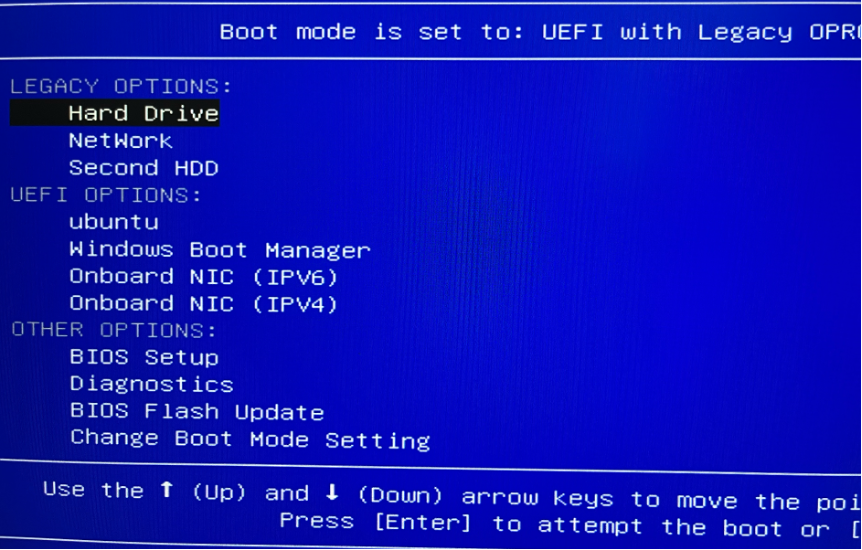
\includegraphics[scale=0.5]{pict/Picture2.png}
    \caption{Boot Menu For Windows}
    \end{centering}
\end{subfigure}
 \begin{subfigure}{.45\textwidth}
    \begin{centering}
    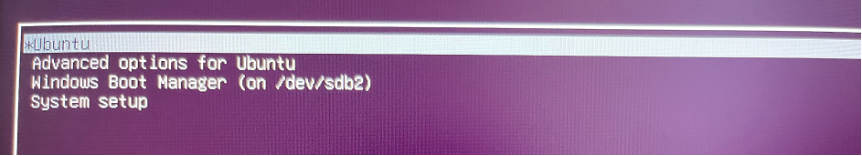
\includegraphics[scale=0.5]{pict/Picture3.png}
    \caption{Boot Menu For Windows}
    \end{centering}
\end{subfigure}
\begin{subfigure}{.5\textwidth}
    \begin{centering}
    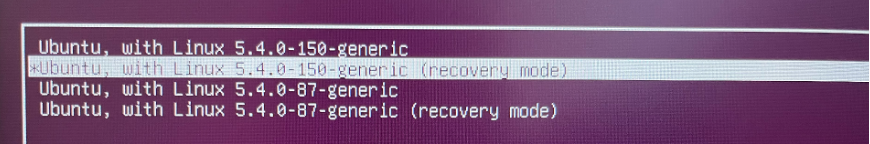
\includegraphics[scale=0.5]{pict/Picture4.png}
    \caption{Advanced Option For Ubuntu}
    \end{centering}
\end{subfigure}
\caption{Reconnaissance, part one}
    \label{fig:1}
\end{figure}

Figure~\ref{fig:1}(a) displays a roster of users who have historically logged into the computer's
desktop offering insights into individuals with access credentials to these systems. This list
serves as a starting point for deeper investigations into the digital footprints these users may have
left online whether through inadvertent postings or publicly shared information that could
potentially be leveraged to gain system access. Additionally, understanding who these users
are opens avenues for direct engagement where strategic social engineering techniques could be
employed to acquire login details, especially in scenarios where direct system infiltration proves
challenging.
% \begin{figure}
%     \centering
%     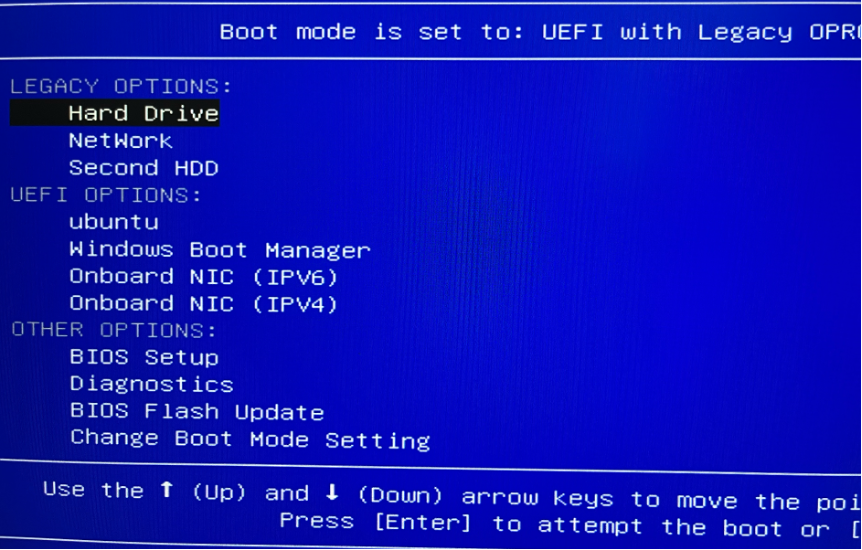
\includegraphics[scale=0.5]{pict/Picture2.png}
%     \caption{Boot Menu For Windows}
%     \label{fig:2}
% \end{figure}

Figure~\ref{fig:1}(b) illustrates the Windows boot menu that surfaces during the system's startup
sequence triggered by pressing F12 at boot time. This item's appearance is rooted in the
Dell desktop computer's underlying Windows architecture despite Ubuntu being the primary
operating system in use. Consequently, adjusting settings within this Windows-centric
menu is unlikely to facilitate access to the system as the critical data and functionalities reside
within the Ubuntu environment. Within the realm of UEFI options presented, selecting the
Ubuntu option emerges as the most effective course of action, as it directly navigates to the
Ubuntu boot menu aligning with the system's operational framework and providing the relevant
access points for system interaction.
% \begin{figure}
%     \centering
%     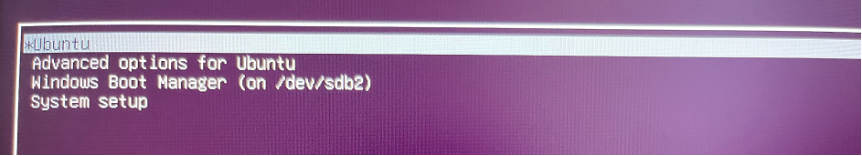
\includegraphics[scale=0.5]{pict/Picture3.png}
%     \caption{Boot Menu For Ubuntu}
%     \label{fig:3}
% \end{figure}
Figure~\ref{fig:1}(c) showcases the Ubuntu boot menu interface which becomes accessible after
choosing the UEFI option from the initial Windows boot menu during the penetration testing
process. This menu offers four distinct choices: the primary Ubuntu option, which leads to
the login screen signaling readiness for user access; Advanced Options which provides
capabilities for managing different Linux versions; the Windows Boot Manager option a pathway that returns the user to the preceding Windows boot menu; and the System Setup
enabling adjustments and configurations within the system's settings. In this boot menu,
there also is the option to edit the command GRUB settings for each of the boot options or to
access the GRUB terminal to make changes to these bootloaders.
% \begin{figure}
%     \centering
%     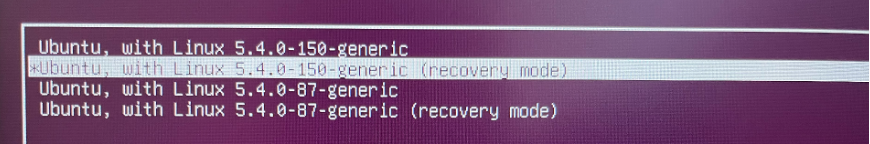
\includegraphics[scale=0.5]{pict/Picture4.png}
%     \caption{Advanced Options For Ubuntu}
%     \label{fig:4}
% \end{figure}
Figure~\ref{fig:1}(d) showcases the advanced options within the Ubuntu boot menu during the
penetration test. This menu offers a selection of Linux Ubuntu versions that can be initiated
via the GRUB bootloader, presenting a crucial step for deeper system analysis. Notably, the
recovery mode option stands out as particularly significant for advancing the reconnaissance
phase of a penetration test. Accessing recovery mode minimizes the need for extensive
administrator credentials, providing a strategic avenue for attempting system access with limited
information, thereby enhancing the tester's ability to probe the system's defenses effectively.
\begin{figure}
    \centering
   \begin{subfigure}{.45\textwidth}
    \begin{centering}
    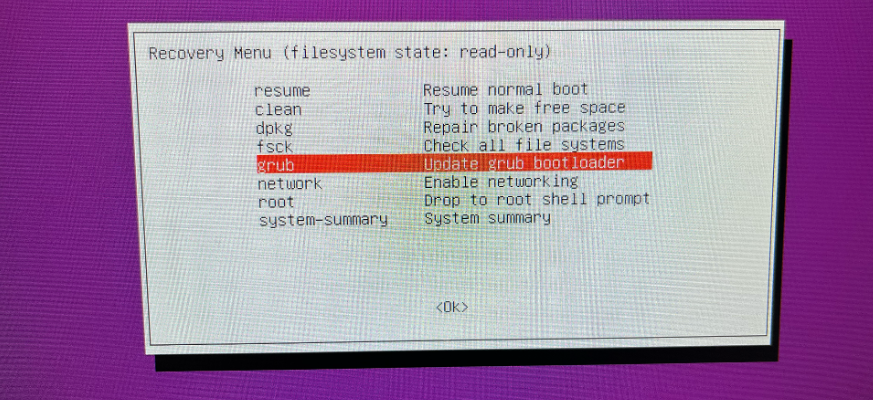
\includegraphics[scale=0.5]{pict/Picture5.png}
    \caption{Ubuntu Linux Recovery Mode}
    \end{centering}
\end{subfigure}
\begin{subfigure}{.5\textwidth}
    \begin{centering}
    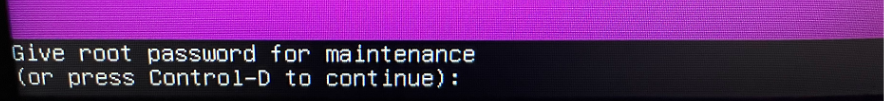
\includegraphics[scale=0.5]{pict/Picture6.png}
    \caption{Attempting To Gain Access To Root Shell Prompt}
    \end{centering}
\end{subfigure}
\caption{Reconnaissance, part two}
    \label{fig:2}
\end{figure}
% \begin{figure}
%     \centering
%     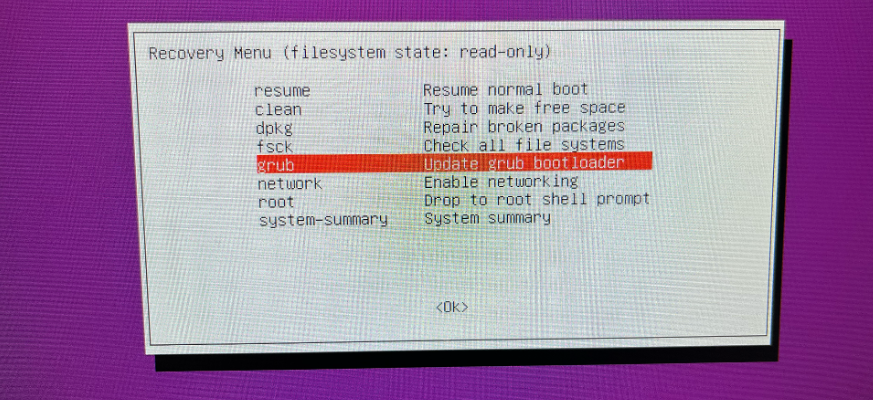
\includegraphics[scale=0.5]{pict/Picture5.png}
%     \caption{Ubuntu Linux Recovery Mode}
%     \label{fig:5}
% \end{figure}

Figure~\ref{fig:2}(a) unveils the recovery mode accessed through the advanced options in the Ubuntu
boot menu a critical feature enabled by the GRUB bootloader. This mode presents a suite of
powerful tools for the security researcher offering capabilities like repairing damaged packages,
conducting file system checks, updating the GRUB loader, enabling network functionalities,
accessing a root shell prompt, and summarizing system status. Each of these functions opens
potential vectors for system manipulation, enhancing the researcher's arsenal for penetration testing. The recovery mode's expansive toolkit raises significant security considerations. For instance, the ability to repair broken packages can be exploited to modify or replace
system files with compromised versions subtly granting unauthorized access. Enabling
networking from recovery mode could allow an attacker to download additional tools or
exfiltrate data without the normal user-level restrictions. Perhaps most potent is the access
to a root shell prompt offering unfettered control over the system to knowledgeable
individuals. This level of access enables a security researcher or an attacker to bypass
standard authentication mechanisms, alter system configurations, and potentially implant
malicious software without detection.
% \begin{figure}
%     \centering
%     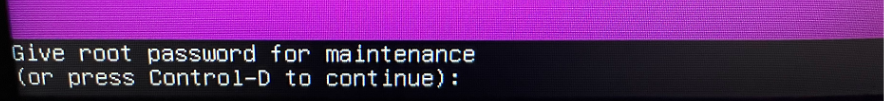
\includegraphics[scale=0.5]{pict/Picture6.png}
%     \caption{Attempting To Gain Access To Root Shell Prompt}
%     \label{fig:6}
% \end{figure}

Figure~\ref{fig:2}(b) reveals the interface presenting a root prompt, encountered when a user
navigates through the advanced options within the Ubuntu recovery mode. This interface is
a testament to the robust security measures integrated into the machine's operating system setup.
Functioning as a critical safeguard this root prompt establishes a formidable obstacle for
potential adversaries compelling them to devise alternative strategies to access a terminal for
executing modifications. The prompt requires the entry of the root password to proceed
with any maintenance activities or to utilize the recovery options emphasizing the system's
commitment to securing privileged operations and thwarting unauthorized access attempts.
This security layer underscores the operating system's design philosophy prioritizing the
protection of sensitive functionalities and ensuring that only authorized users can perform critical
system interventions full security is never possible even when tough to spot.


\subsection{Gaining Access}
Transitioning into the gaining access phase marks a climactic shift in the penetration
testing process where the focus moves from gathering intelligence to actively seeking entry into
the target system using all vulnerabilities that might have been discovered.
Through examination and reconnaissance of the system's landscape this stage leverages the
insights gained to identify and exploit vulnerabilities. In this instance, the tester
applies specialized techniques and tools to breach the system's defenses aiming to secure a
foothold within the environment such as through a backdoor into the system. This
could involve exploiting software vulnerabilities, leveraging misconfigurations, or employing
social engineering tactics. Achieving access is critical, as it allows the tester to
evaluate the system's resilience to attacks simulating the actions of a potential attacker but with
the intent of strengthening the system's security defenses.

\subsubsection{ Getting Access To Terminal}
A key progression in the stages of gaining access to an operating system when
performing penetration testing is the successive infiltration of a terminal on the system since this
can allow a user to perform a plethora of potential security dangers. This access is
pivotal as it lays the foundation for executing commands directly within the system's heart
allowing for a more granular exploration of its vulnerabilities possibly within the version of
Ubuntu. Achieving terminal access marks a significant step enabling the
penetration tester to apply insights gathered during reconnaissance to utilize specific
vulnerabilities or misconfigurations to gain a foothold. This step is about
precision and adaptability navigating through the system's defenses with the dual aims of
highlighting security gaps and reinforcing the system against actual threats.
\begin{figure}
    \centering
   \begin{subfigure}{.7\textwidth}
    \begin{centering}
    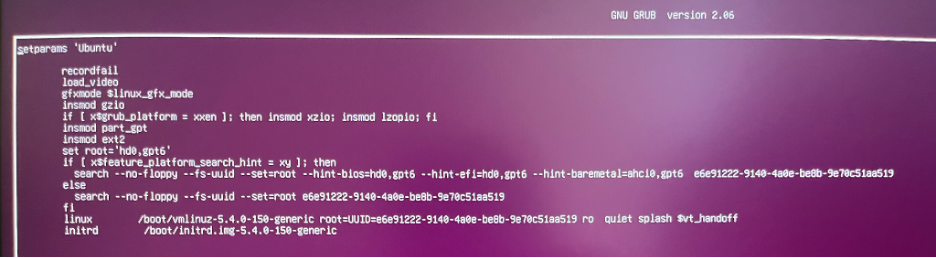
\includegraphics[scale=0.5]{pict/Picture7.png}
    \caption{Editing The Grub Menu For Ubuntu To Gain Terminal Access}
    \end{centering}
\end{subfigure}
\begin{subfigure}{.7\textwidth}
    \begin{centering}
    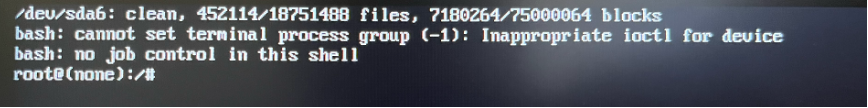
\includegraphics[scale=0.5]{pict/Picture8.png}
    \caption{Saving Using F10 Booting To Root Shell}
    \end{centering}
\end{subfigure}
\begin{subfigure}{.7\textwidth}
    \begin{centering}
    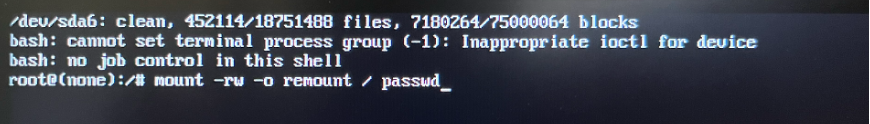
\includegraphics[scale=0.5]{pict/Picture9.png}
    \caption{Mounting The passwd Directory}
    \end{centering}
\end{subfigure}
\begin{subfigure}{.45\textwidth}
    \begin{centering}
    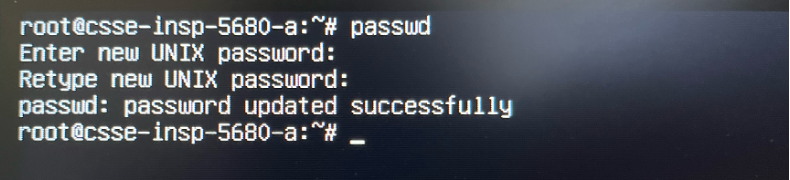
\includegraphics[scale=0.5]{pict/Picture10.png}
    \caption{Changing The Root Password With passwd}
    \end{centering}
\end{subfigure}
\begin{subfigure}{.5\textwidth}
    \begin{centering}
    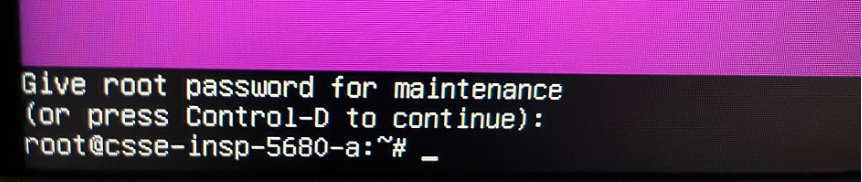
\includegraphics[scale=0.5]{pict/Picture11.png}
    \caption{Logging Into The Root Shell Prompt}
    \end{centering}
\end{subfigure}
\caption{Gaining Access}
    \label{fig:3}
\end{figure}

% \begin{figure}
%     \centering
%     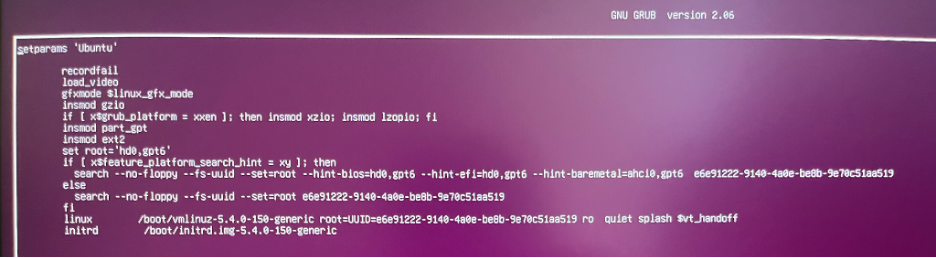
\includegraphics[scale=0.5]{pict/Picture7.png}
%     \caption{Editing The Grub Menu For Ubuntu To Gain Terminal Access}
%     \label{fig:7}
% \end{figure}
Figure~\ref{fig:3}(a) showcases the GRUB loader's editorial interface for Ubuntu accessible from the
boot menu shown in Figure~\ref{fig:1}(c)~\cite{linux,ubuntu,bash1,bash2}. This interface is particularly significant during the boot
process as it outlines the configurations for the Linux distribution set to take effect upon system
restart. These settings are pivotal for system booting enabling modifications to Linux's
configuration without requiring user login. A critical element for the penetration test
highlighted in this context is the line referencing Linux's /boot/volume. This becomes
a focal point for potential exploitation especially when considering the addition of
init=/bin/bash" at the end of this line. Such an alteration manipulates the boot process
compelling the operating system to launch a command prompt with root privileges directly from
the GRUB menu. The implications of this exploit are profound offering unrestricted
access to modify the system's configurations and data. This method represents a
significant security vulnerability granting an attacker comprehensive control over Dell
desktop computer with a single command.
% \begin{figure}
%     \centering
%     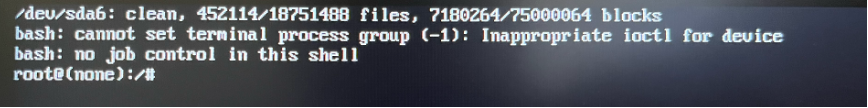
\includegraphics[scale=0.5]{pict/Picture8.png}
%     \caption{Saving Using F10 Booting To Root Shell}
%     \label{fig:enter-label}
% \end{figure}
Figure~\ref{fig:3}(b) captures the moment of access to a command line interface a direct consequence
of modifying the GRUB menu to alter the Linux boot process\cite{bash1,bash2}. This strategic update
compels the system to initiate a command line environment upon startup bypassing standard
security measures and user authentication protocols. Such access provides an unparalleled
opportunity to probe and manipulate the system's settings and data from a position of elevated
privilege. This environment being loaded shows a key exploit that can be taken advantage
of by an adversary if given the opportunity with extensive knowledge of the power this tool
holds. When performing a security test it is crucial to test the limits of these vulnerabilities
to the limit within the scope of the test to ensure that all defenses can be configured to defend
against the attacks performed by the security researcher.

\subsubsection{ Changing Root Password}
Furthering into the access phase, the changing of the root password of a machine
represents a serious maneuver within the penetration testing sequence due to its vital importance
in the system\cite{HackerOne}. This action involves the tester utilizing their obtained terminal access to
modify the system's root password effectively demonstrating the level of control they have
achieved over the system. By altering the root password, the tester not only proves the
vulnerability of the system's most privileged account but also illustrates a potential risk where an
unauthorized user could gain ultimate control over the system's operations. This act
serves both as a proof of concept for the penetration tester and as a stark warning for the system's
administrators, highlighting the critical need for robust security measures to prevent such
unauthorized access. The modification of the root password, while reversible in the
context of ethical penetration testing defines the importance of the cybersecurity field for
protecting systems worldwide.
% \begin{figure}
%     \centering
%     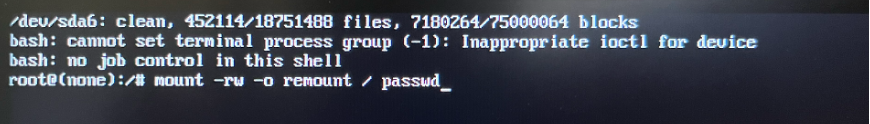
\includegraphics{pict/Picture9.png}
%     \caption{Mounting The passwd Directory}
%     \label{fig:9}
% \end{figure}
Figure~\ref{fig:3}(c) delves deeper into the sequence of modifying the root password a task
undertaken after securing root access via adjustments made in the GRUB loader from Ubuntu's
boot menu. The depicted command initiates the process by targeting the system's passwd
directory which stores the root password. By employing the remount option in the
command line the directory is made accessible with read and write permissions thus granting the
user comprehensive authority to modify any aspect of this directory. This capability to alter
the passwd directory is a critical juncture in the process as it directly impacts system security by
allowing changes to the root password. Such changes can cement the user's control over the
system facilitating further exploration or testing within the machine.
% \begin{figure}
%     \centering
%     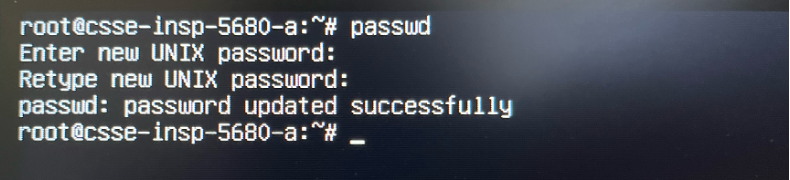
\includegraphics{pict/Picture10.png}
%     \caption{Changing The Root Password With passwd}
%     \label{fig:10}
% \end{figure}

Figure~\ref{fig:3}(d) illustrates the process of altering the root password through a commandeered
command line interface achieved by exploiting root access granted via modifications made in the
GRUB loader from the Ubuntu boot menu. Utilizing the passwd command the intruder is
presented with the opportunity to redefine the root password effortlessly given that the relevant
directory has been mounted with read-write permissions by the attacker. This command
prompts the user to input a new UNIX password followed by a verification step to confirm the
password matches upon re-entry. The successful execution of this command culminates in
the system-wide update of the root password all executed without the necessity for conventional
login procedures. This maneuver exposes significant vulnerabilities within the operating
system's security framework underscoring the urgent need for enhancements to protect user data
effectively. Furthermore, the versatility of the passwd command extends beyond the root
account enabling the alteration of passwords for any user account on the system. This
capability hands the adversary complete control over the system and access to all user accounts
accentuating the critical necessity for implementing stringent security defenses to safeguard
against such unauthorized access and ensure the confidentiality of stored information.

% \begin{figure}
%     \centering
%     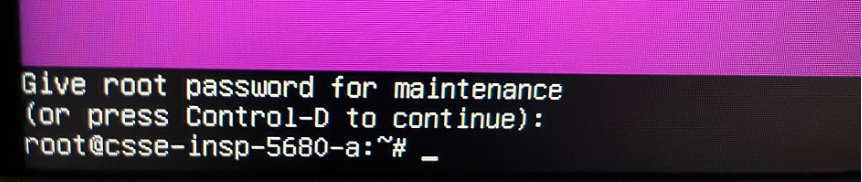
\includegraphics{pict/Picture11.png}
%     \caption{Logging Into The Root Shell Prompt}
%     \label{fig:11}
% \end{figure}
Figure~\ref{fig:3}(e) showcases the ability to log into the root shell prompt that was displayed from
the advanced Ubuntu boot options in the recovery mode of the Linux system as shown in Figure~\ref{fig:2}(b). This displays the full extent of the damage that could be done due to this simple
vulnerability within the Ubuntu operating system that could leave the company in serious
distress if exploited by a knowledgeable adversary since depending on what this system is
hooked up to this could affect complete servers or vital systems.

\subsection{ Maintaining Access}
Once access has been successfully gained the subsequent phase followed requires
maintaining access which becomes crucial in the penetration testing lifecycle. This stage is about establishing a persistent presence within the vital systems enabling ongoing
access for further analysis and testing. Techniques used during this phase may
include creating backdoors, scheduling tasks for automatic re-entry, or exploiting the system's
features to ensure continued access. The objective here is not to cause harm or to
remain undetected by the system's legitimate users but to simulate an attacker's ability to
maintain access over time, thereby identifying and mitigating potential security weaknesses. Becoming undetected within the system also involves dodging the anti-virus on the
operating system or installed on the system if programmed since this may cause inconspicuous
activity when noticing reverse shells or backdoors creating another obstacle for adversaries. This process involves a careful balance of stealth and stability ensuring that the
methods used do not disrupt the system's normal operations or alert the administrators to the
tester's presence.

\subsubsection{Creating A User}
The phase dedicated to maintaining access involves strategic actions to ensure persistent
entry with creating a user being a pivotal tactic. This step is akin to establishing a
secret backdoor into a system since it is a discrete method that allows for re-entry even after the
initial path of access might be discovered and closed by the system's defenders.
The creation of a new user account by the penetration tester is executed often with minimal
privileges to avoid detection yet enough to guarantee a foothold within the system. This maneuver is not about overt control but ensuring a stealthy reliable point of access for
ongoing assessment and monitoring.
\begin{figure}
    \centering
    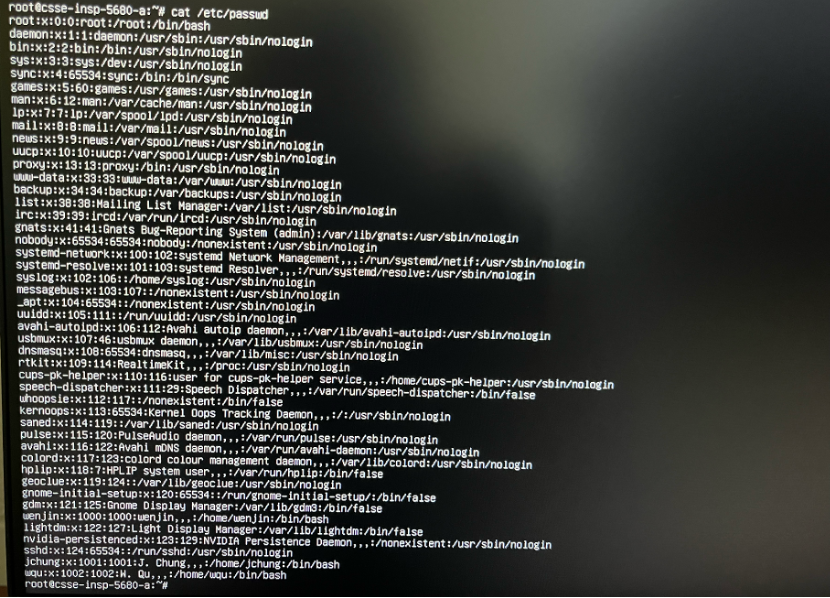
\includegraphics{pict/Picture12.png}
    \caption{Displaying All Users On The System}
    \label{fig:12}
\end{figure}
Figure 12 utilizes the command line interface accessed in Figure 11 to perform an
analysis of all of the active users on the machine to ensure that a created user can properly blend
in with the functional users. The command used to check the active users of the machine is
cat /etc/passwd which is a way to print the directory of passwd thus showcasing all of the users
within the system.
\begin{figure}
    \centering
    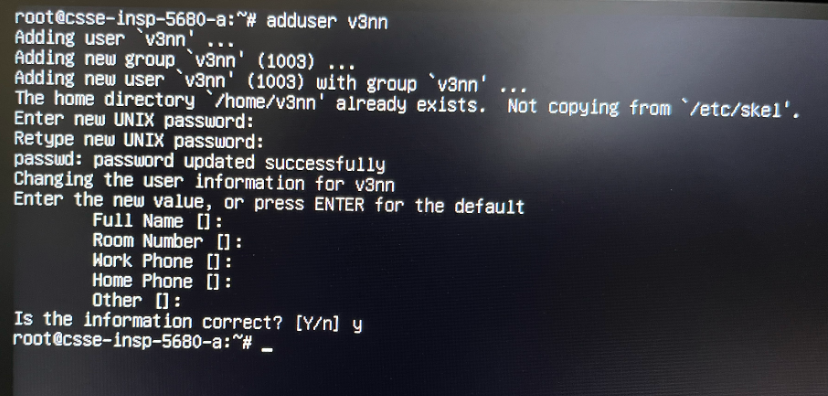
\includegraphics{pict/Picture13.png}
    \caption{Creating A New User}
    \label{fig:13}
\end{figure}
Figure~\ref{fig:13} once again utilizes the command line access gained from Figure~\ref{fig:3}(e) after
getting the root password which here showcases creating an active user on the machine. In
this instance, the command adduser v3nn was used which adduser is used to add a user to the
system and v3nn is the name that will be declared that it is under. The adversary is then
prompted for a password and information which in this case was skipped but in a real scenario a
security researcher might want to match the system organization format and input fake
information for this section to blend in to avoid detection for longer periods of time. The
information is then confirmed and the user is added to the accounts for the system giving them
access at leisure.
\begin{figure}
    \centering
    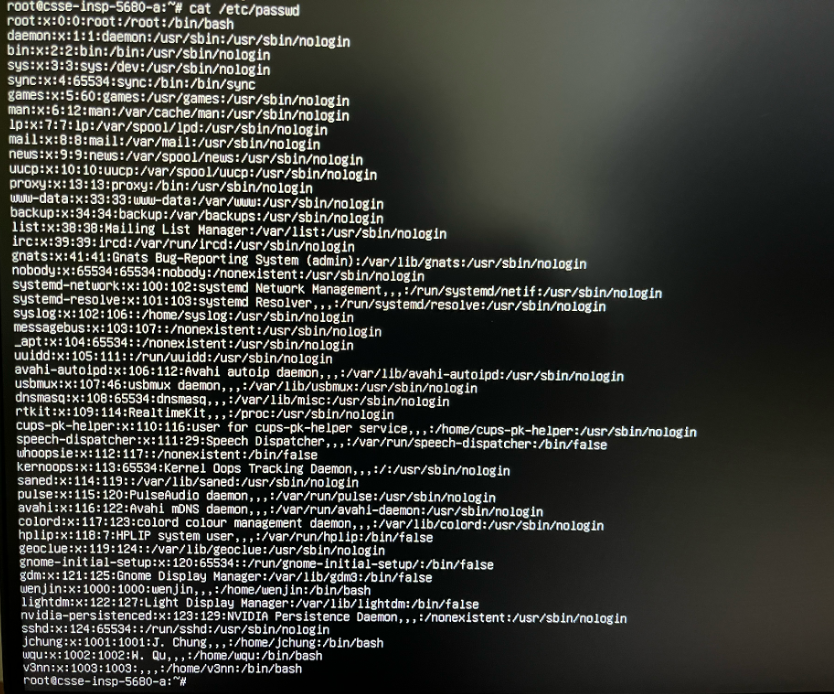
\includegraphics{pict/Picture14.png}
    \caption{Displaying The New List Of Active Users}
    \label{fig:14}
\end{figure}


Figure~\ref{fig:14} illustrates the new list of active users on the system after the adduser command
was executed on the command line in Figure~\ref{fig:13}. This is done using the same command as
in Figure~\ref{fig:12} where cat /etc/passwd is used to print the standard output of all the active users on
the machine. This now displays the user v3nn which was created in Figure~\ref{fig:13} which now
has a userid and information to log in with command line access with minimal privileges.

\subsubsection{Logging In As Created User}
Once a new user account has been strategically established within the target system the
subsequent step involves logging in as this created user testing the ability to maintain access
subtlety within the system. By utilizing the credentials of the newly created user, the tester
not only validates the success of their previous actions but also ensures a level of anonymity and
minimal footprint within the system.
\begin{figure}
    \centering
    
\includegraphics{pict/Picture15.png}
    \caption{Logging In As Created User}
    \label{fig:15}
\end{figure}

Figure~\ref{fig:15} presents the test of the login credentials created through the root command line
access gained from the previous figures using the password and name from the adduser
command in Figure~\ref{fig:13}. In this login stage, the adversary could also log in as the root user
since it has been changed and the user name is just root so once accessed they are able to make
changes without detection since the root user could be anyone on the system only with the
capability of making all system administrator changes.
\begin{figure}
    \centering
    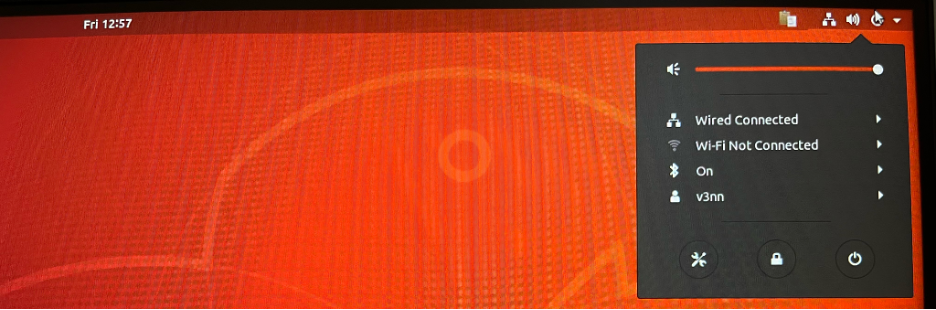
\includegraphics{pict/Picture16.png}
    \caption{Displaying The Created User Logged In}
    \label{fig:16}
\end{figure}
Figure 16 showcases one of the key end goals of the penetration test which was to gain
unauthorized access to the system without login credentials which was done through the stages
of a penetration test. The created user is logged in as can be seen in the top right corner of
the figure in which it displays the user’s name which is v3nn. This unauthorized access shows a
clear vulnerability in the system and now more damage can be done within the system.

\subsubsection{Creating A Backdoor}
In the critical phase of maintaining prolonged access within a penetration test, the
creation of a backdoor stands out as a strategic maneuver. This procedure involves
embedding a covert pathway within the target system enabling seamless re-entry for the tester
without the need for repetitive breach efforts. Essentially, it’s like discreetly planting
a hidden key to the back gate of a fortified castle allowing unobstructed access at will. This backdoor is intricately designed to evade detection by conventional security measures
such as system checks or malware detectors ensuring that the tester can gather necessary data,
monitor system activities, or further assess vulnerabilities over time. The objective
here is not to compromise the system’s integrity but to highlight potential security gaps that
could be exploited by malicious entities.
\begin{figure}
   \begin{minted}{c}
REM Title: Execute Backdoor Access
REM Author: V3NN
REM Description: Opens Terminal, writes, executes, and deletes a bash script.
REM Declare the attackmode to be used for storage and human interface device
ATTACKMODE HID STORAGE
DELAY 1000

GUI SPACE
DELAY 200
STRING Terminal
DELAY 200
ENTER
DELAY 1000
STRING echo "mkfifo /tmp/f; cat /tmp/f | /bin/sh -i 2>&1 | nc 192.168.1.10 4444 > /tmp/f" > /tmp/script.sh
DELAY 200
ENTER
STRING chmod +x /tmp/script.sh
DELAY 200
ENTER
STRING rm /tmp/script.sh
DELAY 200
ENTER
STRING exit
DELAY 200
ENTER
\end{minted}
    \caption{Code Segment 1. Sample Code For Setting Up Reverse Shell Using Rubber Ducky}
    \label{fig:enter-label}
\end{figure}
This script tailored for the USB Rubber Ducky automates the process of opening a terminal on a macOS system and establishes a covert backdoor for remote infiltration. Initially, the script employs the GUI SPACE command to open Spotlight then types "Terminal" to launch it simulating user actions to start a terminal session. The core of the script involves creating and executing a Bash script named /tmp/script.sh that initiates a reverse shell connection to a specified IP address on port 4444. This effectively grants the ability to remotely execute commands on the target machine. The script ensures that the Bash file is executable and then immediately deletes it to remove any trace of the operation, concluding with an exit from the terminal to maintain stealth. This approach not only sets up a persistent backdoor but also cleans up after itself to avoid detection.

\begin{figure}
   \begin{minted}{c}
nc -lvnp 4444
\end{minted}
    \caption{Code Segment 2. Command For Netcat Running On Host Machine}
    \label{fig:enter-label}
\end{figure}
Code Segment 2 presents the command nc -lvnp 4444 which is a crucial command to run
on the attacker's host machine for Code Segment 1 to properly execute keeping in mind this is
not part of the Rubber Ducky script. It uses Netcat to listen on port 4444 for the
incoming reverse shell connections from the target machine placed at the attacker IP address
ready to receive the shell once the backdoor script executes. This setup illustrates a
sophisticated method of gaining unauthorized access to a system showcasing the potential danger
for seemingly innocuous devices to execute malicious operations covertly on a network within
homes, businesses, or even schools.

\subsection{Covering Tracks}
In the final phase of penetration testing known as Covering Tracks, the focus shifts
towards erasing any digital footprints that could betray the presence or actions of the tester
within the system. This phase is crucial since this would resemble the careful
steps a bad actor might take to ensure no evidence is left behind after they have infiltrated the
system pocketing the prize. By meticulously removing logs, histories, and any
temporary files created during the testing process the tester safeguards against the detection of
their activities. This action is not only a demonstration of technical proficiency
but also an adherence to ethical standards ensuring that the system remains secure and
undisturbed post-assessment. Additionally, this phase underlines the importance
of non-disruption in penetration testing reinforcing the principle that the aim is to strengthen
security without compromising the integrity or functionality of the target system.
Covering tracks is thus a testament to the tester's skill in navigating the system invisibly leaving
it as they found it secure against future threats with no trace of their entry or exploration.

\subsubsection{ Deleting System Logs \& Command History}
Within the nuanced process of ensuring a clean and undetectable exit from a system postpenetration testing the deletion of system logs and command history emerges as a critical step. This meticulous action mirrors the precision of an expert cleaner who leaves no trace of their
work safeguarding the integrity of the environment they've interacted with.  By carefully
erasing these digital breadcrumbs the tester effectively obscures their movements and
interventions within the system preventing any potential discovery of their access or the methods
employed.
\begin{figure}
    \centering
    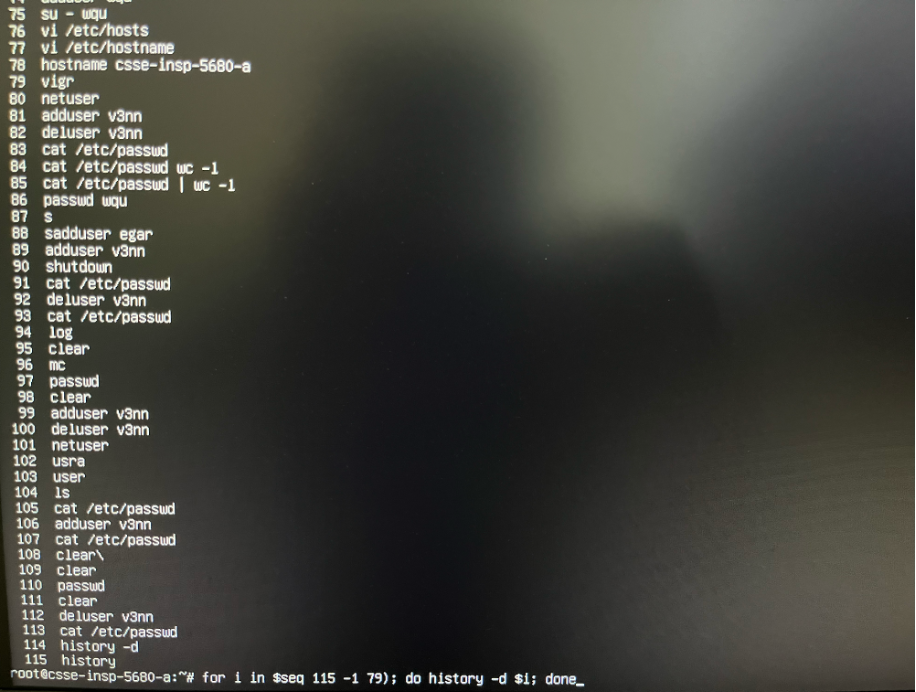
\includegraphics{pict/Picture17.png}
    \caption{Deleting The Shell Logs Of Commands}
    \label{fig:17}
\end{figure}
Figure~\ref{fig:17} displays the deleting of shell logs from the command line of the root used to
create, delete, and add users as well as change the root password for the machine.
The method used in this figure for deleting logs is using a BASH for loop to sequentially repeat
the history -d command which deletes the history for a line number listed to the left of a
command. This goes through all of the commands from 79 to 115 deleting each of
the commands leaving no trace of the effects of these commands. The alternative to
this method could be to delete the log files and ensure all of the changes made to the system have
been reverted to ensure no damage has been done to the machine.

\subsection{Lessons learned from penetration testing engagements}
The penetration testing process performed on the Ubuntu Linux operating system reveals insights into system vulnerabilities and defense strategies. First and foremost, the process underscores the importance of regular checks on system configurations and access controls by users and non-users. The exploitation of the GRUB loader to gain root access without a password illustrates a significant vulnerability point that could be mitigated by securing the bootloader settings along with using encrypted passwords. Additionally, the ease with which the root password can be changed needs to be altered so that the machine is less vulnerable to becoming compromised completely without authorization. Having the ability to create new users with given access highlights the need for robust monitoring systems to detect and alert unauthorized changes to user accounts or group privileges. This engagement also stresses the necessity of maintaining updated and patched systems to minimize vulnerabilities and reduce the attack surface available to potential adversaries. Furthermore, the effectiveness of physical security measures such as securing USB ports to prevent Rubber Ducky attacks is a critical reminder of the need for comprehensive security protocols that address both digital and physical threat vectors.

\section{On Windows}
In penetration testing, both Linux and Windows provide mechanisms to access command prompts through recovery modes although utilizing different methods. While Linux utilizes the GRUB bootloader for direct system setting manipulations via the boot menu, Windows systems often leverage a technique within the System32 directory. Specifically, this involves renaming utilman.exe to cmd.exe which allows unauthorized users to access the command prompt directly from the login screen by triggering the ease of access center bypassing login credentials. This method was successfully executed on a Windows 7 professional edition machine highlighting potential security vulnerabilities. However, attempts to replicate this on a Windows 10 machine were thwarted by a password-protected command prompt in recovery mode indicating enhanced security measures that block access to the System32 directory and safeguard against such exploits. The effectiveness of this approach varies across Windows versions from 7 to 11 largely depending on how security features are configured. This emphasizes the critical need for robust security configurations and ongoing system updates to prevent unauthorized access in Windows environments.

\section{Challenges and Future Trends}
\paragraph{Anticipating how emerging technologies (e.g., cloud computing, IoT) will impact OS security}
Emerging technologies like cloud computing and the Internet of Things (IoT) are rapidly expanding the security boundaries traditionally managed by operating systems. The integration of cloud services has introduced complex challenges in securing data that traverses multiple environments requiring operating systems to become more versatile and secure in regards to data integrity and privacy. Similarly, IoT devices extend the operating system's reach into everyday objects such as smart fridges, washing machines, to even toothbrushes all connected to the internet providing a potential vulnerability for an attacker to gain access to your network. These devices often operate with minimal security increasing the need for scalable security measures embedded within the OS to manage threats across highly heterogeneous networks. On a similar note, there are even IoT devices that might be inconspicuous to attackers that could be highly dangerous if attacked such as major healthcare devices used in hospitals for things such as surgeries, maintaining patients' life support and medicine, or every other crucial system in healthcare. Many of these devices work off some sort of operating system or some sort of framework which if not updated and tested regularly could be a potential breach by an attacker that could lead to major repercussions.

\paragraph{The importance of continuous learning and adaptation for penetration testers due to the evolving threat landscape}
As the technology evolves along with it comes the advanced complexity of threats making continuous learning and adaptation essential for penetration testers. This dynamic field demands a proactive approach to security where knowledge of the latest vulnerabilities, attack vectors, and mitigation strategies is critical to the success of finding vulnerabilities in systems before adversaries. Penetration testers must regularly update their skills and tools used to anticipate and counteract emerging threats of hackers. Engaging with the cybersecurity community in forums, events, and participating in ongoing training. Staying up-to-date on new research is vital for maintaining the effectiveness of security measures and ensuring that security practices evolve in step with the rapidly changing digital environment. This relentless pursuit of knowledge not only enhances a tester’s capability to protect systems but also fortifies the overall security posture of the organizations they defend.

\section{Conclusion}
Penetration testing plays a pivotal role in enhancing operating system security serving as a proactive measure to identify and mitigate potential vulnerabilities before they can be exploited by an adversary. This practice is essential not only for the integrity of the operating systems but also for safeguarding the broader digital infrastructure of organizations. By simulating attacks, penetration testers can reveal weaknesses in security architectures, contributing significantly to the overall security posture of organizations. This, in turn, ensures the protection of end-user data against increasingly sophisticated cyber threats. Ultimately, regular and rigorous penetration testing is indispensable for maintaining robust defense mechanisms in today's dynamic threat landscape.

\clearpage

\bibliographystyle{plainnat}
\bibliography{main}

\end{document}
\endinput
%%
%% End of file `sample-authordraft.tex'.
